\documentclass[11pt,a4paper]{article}
\usepackage[utf8]{inputenc}
\usepackage[T1]{fontenc}
\IfFileExists{lmodern.sty}{\usepackage{lmodern}}{}
\usepackage[margin=2.3cm]{geometry}
\usepackage{amsmath,amssymb,bm}
\usepackage{graphicx}
\usepackage{booktabs}
\usepackage{xcolor}
\usepackage{caption}
\usepackage{enumitem}
\usepackage[hidelinks]{hyperref}
\usepackage{xurl}
\usepackage{float}
\usepackage[most]{tcolorbox}
\newtcolorbox{keybox}[1]{enhanced, colback=blue!5, colframe=blue!60!black, fonttitle=\bfseries, title={#1},
  left=6pt, right=6pt, top=4pt, bottom=4pt}
\graphicspath{{figures/}}
\setlist{itemsep=2pt,topsep=4pt}

\title{\textbf{Flow Reconstruction from Sparse Observations:\\ Step-1 Control for the Mamba Deformation Model}\\[4pt]
\large MS Thesis I --- Report on the experiments requested on 21 November 2026}
\author{Muhammad Hussain Qureshi (MSDS25010)\\
Advisor: Dr.\ Ali Murtaza\\
Faculty of Sciences, Information Technology University, Lahore}
\date{November 24, 2026}

\begin{document}
\maketitle

\begin{abstract}
\noindent We tested whether a Mamba deformation network improves 4D Gaussian reconstruction of 2D Navier--Stokes
vorticity from 10\% of the pixels, against an MLP and a GRU with the same smoothness term, matched network size
($\approx$69k parameters), the same training budget, a smoothness weight tuned for each model on validation frames,
and 5 flows $\times$ 3 seeds. The success criterion was fixed before the runs. \textbf{Mamba does not meet it}: it
beats the MLP by $+2.42$\,dB (95\% CI $[1.61, 3.23]$) but is $-0.46$\,dB ($[-1.73, 0.80]$) behind the GRU. The
earlier gain therefore comes from reading each trajectory in time order with temporal regularisation, not from
Mamba itself. A non-learned baseline (cubic interpolation in space, linear in time) is the best model on test PSNR
(27.36\,dB). Mamba reproduces the energy spectrum best, but overfits the observed pixels.
\end{abstract}

\begin{keybox}{Verdict against the pre-registered criterion}
Criterion (fixed on 22 November, before any run): \emph{Mamba wins if its held-out PSNR is at least 1\,dB higher
than both the MLP and a GRU, averaged over 5 flows $\times$ 3 seeds, with the 95\% CI of each paired difference above
0; all models get the same smoothness term with the weight tuned per model on a validation split, network parameters
within $\pm10\%$, and 3000 iterations each.}

\smallskip
\begin{tabular}{lcc}
Mamba $-$ MLP & $+2.42$\,dB, CI $[+1.61, +3.23]$ & meets \\
Mamba $-$ GRU & $-0.46$\,dB, CI $[-1.73, +0.80]$ & \textbf{does not meet} \\
\end{tabular}

\smallskip
\textbf{Result: Mamba does not win.} The finding is that temporal regularisation (with a recurrent reading of each
trajectory) drives the gain.
\end{keybox}

\section{Setup}
\begin{itemize}
\item \textbf{Data.} InverseBench \texttt{NavierStokes2d}, 2$\pi$-periodic, $128^2$, $Re=200$ (inverse dimensionless
viscosity), forcing $-4\cos(4y)$; 5 initial fields from the InverseBench test set, rolled out for 21 frames at
$\Delta t=0.05$ ($\approx$0.25 eddy turnover times per step, $\omega_{\text{rms}}=4.6$--5.3). Field: vorticity$/10$.
\item \textbf{Observations.} 10\% of the pixels of each frame, drawn independently per frame, the same masks for every
model. Frames 2, 6, 10, 14, 18 are never observed (test). For choosing the smoothness weight, frames 8 and 16 were
also held out (validation) on flows 0--1; the final runs train on all 16 training frames.
\item \textbf{Model.} 2000 canonical 2D Gaussians plus a deformation network that maps (canonical position, $t$) to
offsets of all 6 Gaussian parameters. Loss: masked MSE on observed pixels plus the smoothness term
$\lambda\,\mathrm{mean}\,\lVert\Delta\theta(t{+}1)-\Delta\theta(t)\rVert^2$ on the offsets.
\item \textbf{Networks (matched size).} MLP (width 175, 69{,}131 parameters); GRU (hidden 103, causal over time,
68{,}913); Mamba (2 blocks, $d=64$, causal, 69{,}062). Same inputs, same output head, 3000 Adam iterations each.
\item \textbf{Baselines.} Interpolation: cubic \texttt{griddata} of the observed pixels in each training frame
(periodic), linear interpolation in time for the other frames. Ceiling: all pixels of the training frames observed
(2 flows, 1 seed).
\item \textbf{Metrics.} PSNR (peak-to-peak 2) over all pixels of the test frames; error split into observed pixels,
unobserved pixels of training frames, and test frames; energy spectrum and enstrophy on test frames.
\end{itemize}

\section{Choosing the smoothness weight (validation frames only)}
\begin{table}[H]
\centering
\caption{Mean validation PSNR (dB) on frames 8 and 16, flows 0--1, seed 0. Bold: chosen weight.}
\begin{tabular}{lcccc}
\toprule
$\lambda$ & 0 & 0.3 & 1 & 3 \\
\midrule
MLP   & 22.91 & \textbf{23.16} & 22.82 & 22.67 \\
GRU   & 25.24 & \textbf{25.80} & 25.58 & 25.04 \\
Mamba & 22.26 & 25.32 & \textbf{25.39} & 25.18 \\
\bottomrule
\end{tabular}
\end{table}
\noindent The smoothness term matters most for Mamba ($+3.1$\,dB from $\lambda=0$), little for the GRU ($+0.6$) and
the MLP ($+0.3$). Without it, Mamba is the weakest of the three.

\section{Results}
\begin{table}[H]
\centering
\caption{Final runs, 10\% observed. PSNR in dB; test = the 5 never-observed frames. 15 runs per network
(5 flows $\times$ 3 seeds), 5 for interpolation. ``Observed/unobserved px'' = training frames. Spectrum error = mean
$|\log_{10}(E_{\text{rec}}/E_{\text{true}})|$ for $k\le32$. Time per run on a Kaggle T4.}
\resizebox{\linewidth}{!}{%
\begin{tabular}{lccccccccc}
\toprule
Model & $\lambda$ & Test PSNR & SD flows & SD seeds & Observed px & Unobserved px & Spectrum err. & Enstrophy ratio & min/run \\
\midrule
Interpolation & -- & \textbf{27.36} & 0.89 & -- & exact & 26.38 & 0.421 & 0.929 & 0.01 \\
GRU   & 0.3 & 26.38 & 1.53 & 0.54 & 32.25 & 26.38 & 0.072 & 0.980 & 3.8 \\
Mamba & 1.0 & 25.92 & 0.96 & 0.27 & 36.22 & \textbf{28.89} & \textbf{0.046} & 0.979 & 36.7 \\
MLP   & 0.3 & 23.50 & 1.08 & 0.51 & 28.66 & 24.08 & 0.103 & 0.977 & 3.1 \\
\bottomrule
\end{tabular}}
\end{table}

\begin{table}[H]
\centering
\caption{Test PSNR (dB) per flow, averaged over seeds, and paired differences (t-interval over 5 flows).}
\begin{tabular}{lcccc}
\toprule
Flow & Interpolation & GRU & Mamba & MLP \\
\midrule
0 & 27.90 & 27.59 & 25.82 & 24.29 \\
1 & 27.73 & 26.14 & 25.84 & 23.62 \\
2 & 25.82 & 24.50 & 24.48 & 21.95 \\
3 & 27.38 & 25.44 & 26.33 & 22.97 \\
4 & 27.95 & 28.24 & 27.11 & 24.65 \\
\bottomrule
\end{tabular}

\vspace{6pt}
\begin{tabular}{lccc}
\toprule
Difference & Mean (dB) & 95\% CI & Flows won \\
\midrule
Mamba $-$ MLP & $+2.42$ & $[+1.61, +3.23]$ & 5/5 \\
Mamba $-$ GRU & $-0.46$ & $[-1.73, +0.80]$ & 1/5 \\
GRU $-$ MLP & $+2.88$ & $[+2.24, +3.53]$ & 5/5 \\
Interpolation $-$ Mamba & $+1.44$ & $[+0.78, +2.10]$ & 5/5 \\
Interpolation $-$ GRU & $+0.98$ & $[-0.18, +2.13]$ & 4/5 \\
\bottomrule
\end{tabular}
\end{table}

\begin{figure}[tbp]
\centering
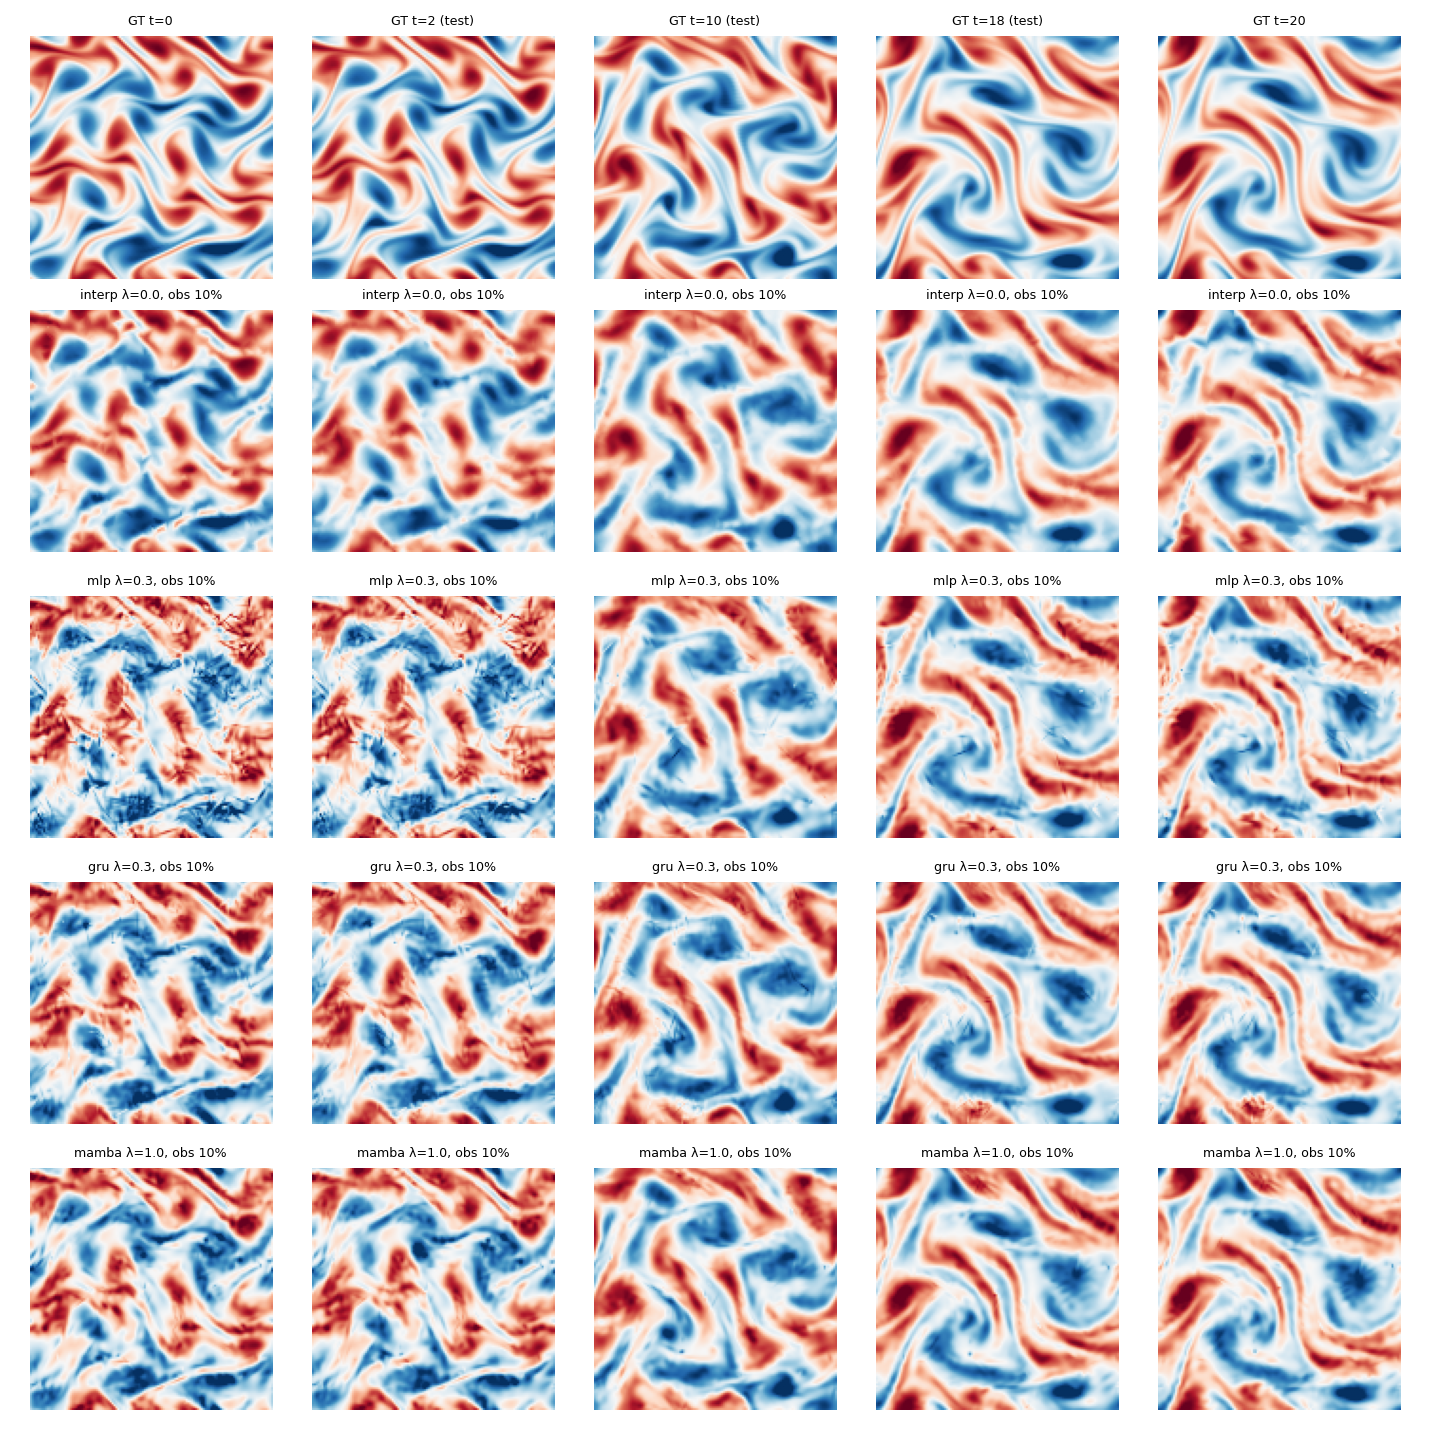
\includegraphics[width=0.78\linewidth]{recon_flow0.png}
\caption{Flow 0, seed 0, 10\% observed. Top row: ground truth; frames 2, 10 and 18 are never observed. Rows below:
interpolation, MLP, GRU, Mamba. The MLP leaves streaks near the start of the window; interpolation is smooth.}
\end{figure}

\begin{figure}[tbp]
\centering
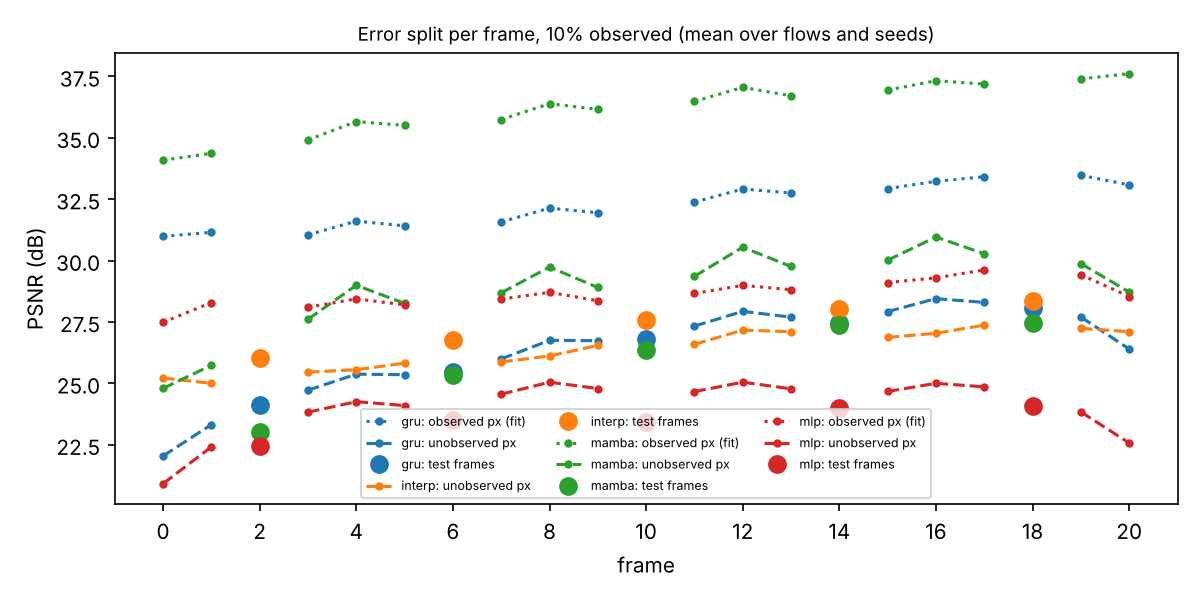
\includegraphics[width=\linewidth]{per_frame.png}
\caption{Error split per frame (mean over flows and seeds): fit on the observed pixels (dotted), unobserved pixels of
training frames (dashed) and test frames (dots). Interpolation reproduces observed pixels exactly (not shown).}
\end{figure}

\begin{figure}[tbp]
\centering
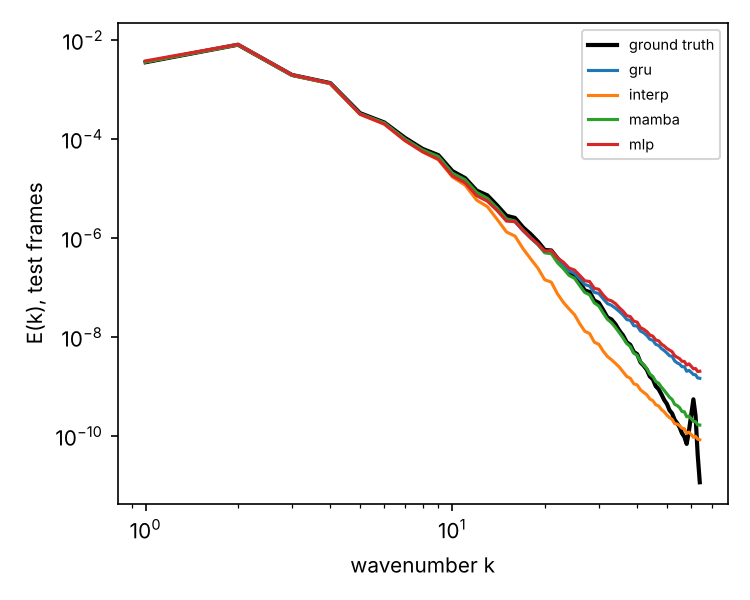
\includegraphics[width=0.55\linewidth]{spectra.png}
\caption{Energy spectrum on the test frames (mean over flows and seeds).}
\end{figure}

\begin{table}[H]
\centering
\caption{Ceiling: all pixels of the training frames observed (2 flows, seed 0). Test PSNR (dB).}
\begin{tabular}{lcccc}
\toprule
& Interpolation & GRU & MLP & Mamba \\
\midrule
Test PSNR & 34.04 & 33.27 & 28.96 & 27.89 \\
\bottomrule
\end{tabular}
\end{table}

\section{Findings}
\begin{enumerate}
\item \textbf{Mamba does not beat a matched GRU.} With the same smoothness term, tuned weights, matched size and
budget, the GRU is 0.46\,dB better on average (not significant) and 10$\times$ faster to train. The earlier
``+2.8\,dB over the MLP'' is real against the MLP, but it belongs to recurrence plus temporal regularisation.
\item \textbf{Interpolation is the strongest baseline on PSNR.} Cubic-in-space, linear-in-time interpolation beats
Mamba on every flow ($+1.44$\,dB) and the GRU on 4 of 5 flows (CI includes 0). At 10\% observation and about a quarter
of an eddy turnover between frames, the flow is smooth enough that a non-learned method is hard to beat.
\item \textbf{Mamba is best on two secondary measures} (not part of the criterion, so exploratory): the spectrum is
closest to the truth (error 0.046 vs.\ 0.072 GRU, 0.103 MLP), and it fills the unobserved pixels of observed frames
best (28.9 vs.\ 26.4\,dB). Interpolation is too smooth beyond $k\approx10$, which PSNR does not penalise much.
\item \textbf{Mamba overfits the observed pixels} (36.2\,dB vs.\ 32.3 GRU) and is the weakest model when all pixels are
observed (27.9\,dB vs.\ 33.3 GRU), which explains why its fill-in quality does not carry over to unseen frames.
\item \textbf{The error at $t=0$ is not underfitting.} At the first and last frames the observed pixels are fitted
well (GRU $\approx$31\,dB, Mamba $\approx$34\,dB); the error is on the 90\% of pixels never seen, at the ends of the
time window, where a causal network has no history.
\end{enumerate}

\section{Consequences and next steps}
\begin{itemize}
\item The flow section will be framed as: \emph{temporal regularisation, with a recurrent reading of each trajectory,
drives the gain; Mamba gives no advantage over a GRU of the same size}, with the interpolation baseline reported
alongside. ``+2.8\,dB over the MLP'' is removed from the slides and poster.
\item As agreed, the observation-rate sweep and longer sequences are not run, since Mamba did not pass step 1.
\item Next: the 3D items (matched-budget control, about 10 volumes $\times$ 2 seeds at 60 receivers, TV-regularised
grid, measurement noise at a stated SNR, tables for the controls) and the related-work additions (4DSTR, Gamba,
Wasserstein-constrained 4DGS).
\end{itemize}

\paragraph{Reproducibility.} Code: \url{https://github.com/muhammadhussainqureshi/thesis-gs} (commit \texttt{baa2de0});
configs \texttt{thesis1\_step1\_a/b.json}; results and logs in \texttt{results/2026-11-24\_step1/}; report script
\texttt{bin/ns4d\_step1\_report.py}. GPU time: 7.8\,h (session A) + 10.4\,h (session B) on a Kaggle T4.

\end{document}
